\documentclass[draft,ras]{Template/AGUTeX}

\usepackage{graphicx}   
\usepackage{setspace}
\usepackage{amsxtra}
\usepackage{amsmath}
\usepackage{amssymb}
\usepackage{multirow}
\usepackage{bm}
\RequirePackage{lineno}
\linenumbers
% graphics path
\graphicspath{{Figs/}}

\authorrunninghead{SWOBODA ET AL.}
\titlerunninghead{Electronic Scanned ISR Analysis}


\authoraddr{Corresponding author: J. P. Swoboda,
Department of Electrical \& Computer Engineering,
Boston University, 8 Saint Mary�s Street
Boston, MA 02215, USA.
(swoboj@bu.edu)}

\begin{document}

\title{Space-Time Ambiguity Functions for Electronically Scanned ISR Applications}
%%%%%%%%%%%%%% Author Info %%%%%%%%%%%%%%%%%%%%%%%%%%%%%%%%%%%%%
\authors{John Swoboda,\altaffilmark{1}
Joshua Semeter,\altaffilmark{1} Philip Erickson \altaffilmark{2}}

\altaffiltext{1}{Department of Electrical \& Computer Engineering,
Boston University, Boston, Massachusetts, USA.}
\altaffiltext{2}{Haystack Observatory, Massachusetts Institute of Technology, Westford, Massachusetts, USA.}
%%%%%%%%%%%%%% Abstract %%%%%%%%%%%%%%%%%%%%%%%%%%%%%%%%%%%%%

\begin{abstract} Electronically steerable array (ESA) technology has recently been applied to incoherent scatter radar (ISR) systems. These arrays allow for pulse-to-pulse steering of the antenna beam to collect data in a three dimensional region. This is in direct contrast to dish based antennas, where ISR acquisition is limited at any one time to observations in a two dimensional slice. This new paradigm allows for more flexibility in the measurement of ionospheric plasma parameters.  

Multiple ESA based ISR systems operate currently in the high latitude region where the ionosphere is highly variable in both space and time. Because of the highly dynamic nature of the ionosphere in this region, it is important to differentiate between measurement induced artifacts and the true behavior of the plasma. Often three dimensional ISR data produced by ESA systems are fitted in a spherical coordinate space and then the parameters are interpolated to a Cartesian grid, potentially introducing error and impacting the reconstructions of the plasma parameters.

To take advantage of the new flexibility inherent in ESA systems, we present a new way of analyzing ISR observations through use of the space-time ambiguity function. The use of this new measurement ambiguity function allows us to pose the ISR observational problem in terms of a linear inverse problem whose goal is the estimate of the time domain lags of the intrinsic plasma autocorrelation function used for parameter fitting. The framework allows us to explore the impact of non-uniformity in plasma parameters in both time and space. We discuss examples of possible artifacts in high latitude situations, and discuss possible ways of reducing them and improving the quality of data products from electronically steerable ISRs.

\end{abstract}

%%%%%%%%%%%%%%  End of Abstract %%%%%%%%%%%%%%%%%%%%%%%%%%%%%%%%%%


\begin{article}

%%%%%%%%%%%%%% Intro %%%%%%%%%%%%%%%%%%%%%%%%%%%%%%%%%%%%%

\section{Introduction}
Incoherent scatter radar (ISR) is a powerful tool for exploring the ionosphere. These systems can give measurements of electron density $N_e$, ion temperature $T_i$, electron temperature $T_e$, ion velocity $V_i$ and other plasma parameters \citep{dougherty:farley1960, farleydougherty:ISR2, doughteryfarley:ISR3, hagfors1961}. These parameters are measured by matching radar measured power spectra to a parameterized first-principles, physics based model of the power spectrum of the signal scattered from random ionospheric electron density fluctuations. Alternatively, fitting can be done in the lag domain by using the intrinsic autocorrelation function (ACF) of the plasma, which can be determined by taking an inverse Fourier transform of the power spectrum\citep{Lehtinen1996435}. 

The spectral measurement process is fundamentally an estimation of a second order statistic of an inherently random process from the scattering of electrons. In order to get an estimate of the ACF with reasonable statistical properties, an ensemble average must be performed by averaging power spectra or autocorrelation functions together from different pulses. With traditional dish antennas, ISR systems build  statistics in a limited number of ways. One method consists of pointing the radar beam in a specific direction and dwelling until enough pulses are integrated to get the desired statistics. Alternatively, the beam can be scanned through a field of view, collecting pulses while moving. These techniques use an implicit assumption about the uniformity of the plasma parameters within a volume defined by the pulse shape and solid angle beam properties while pulses are being integrated. This leads to an assumption of stationarity of the ACF within a temporal and spatial resolution cell of the radar. 

In many cases, especially in the high latitude ionosphere, this stationarity assumption is not met. Phenomena such as polar cap patches can drift at greater than 1 km/s, and thus the residency time of a particular plasma parcel within a radar beam may be much shorter than the integration time required to estimate an ACF \citep{dahlgren2012di}. In the auroral zone, ionospheric variations produced by auroral particle precipitation occur on similarly short time scales compared to the integration period \citep{Zettergren:2008ba}.

Recently, electronically steerable array (ESA) technology has started to be leveraged by the ISR community. The Advanced Modular Incoherent Scatter Radar (AMISR) systems have already been deployed both at the Poker Flat Alaska (PFISR) and Resolute Bay Canada (RISR) geospace facilities. The European led EISCAT-3D project is currently being developed using phased array technology as well and will be capable of multistatic processing. These new systems are already being used in a number of different ways including creating volumetric reconstructions of plasma parameters \citep{Semeter2009738, Nicolls:2007ie, dahlgren2012di,Dahlgren:2012dq}. These reconstructions primarily consist of recasting ISR data into a Cartesian space through interpolation, after parameters have first been fit in a spherical coordinate system. Others have reconstructed full vector parameters using estimates of the ion velocity which can be determined using the Doppler shift of spectra \citep{butler:imagingfregiondrifts,RDS:RDS20195}.

These new ESA based systems differentiate themselves from dish antennas in a fundamental way. Instead of dwelling in a single beam or scanning along a prescribed direction, an ESA can move to a different beam position within its field of view on a rapid, pulse by pulse basis. An illustration of the differences between ESA and conventional radar systems with respect to statistical integration of radar pulses, focusing on time history of beam positions, starts with the desired grid of geographic parameter coverage in Figure \ref{fig:bp1}. Figure \ref{fig:dbsts} shows a possible path for a dish based antenna to cover this measurement space through moves to different beam positions through time, represented on the z-axis as pulse repetition intervals (PRIs). The dish sweeps through the field of view in a continuous scan.  In contrast, an ESA system can instead move from position to position in discrete steps as seen in Figure \ref{fig:phbsts}. We note as well that the phased array antenna is able to collect data from different beams during overlapping time periods, creating a lattice like pattern. This type of pulse-to-pulse beam position change is very difficult to accomplish with dish antenna systems having significant pointing inertia. 

\begin{figure}
	\centering
	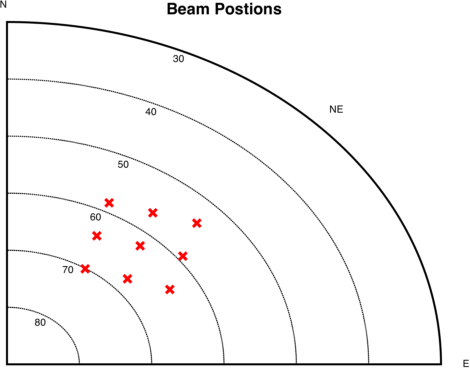
\includegraphics[width=3.5in]{beampositionssts}
	\caption{A 3x3 grid of desired measurement positions in a
          hypothetical geodetic latitude/longitude space. }
	\label{fig:bp1}
\end{figure}

\begin{figure}
	\centering
	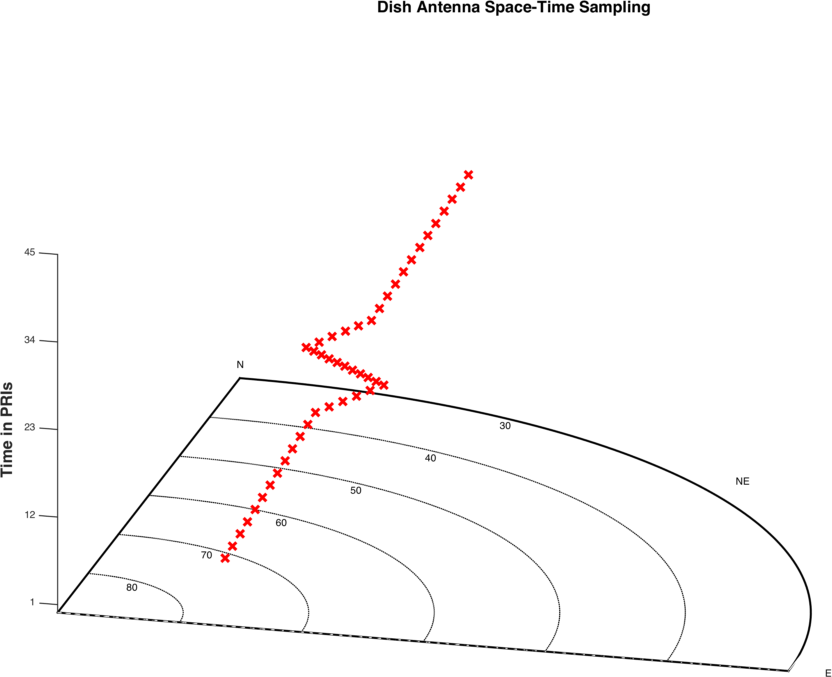
\includegraphics[width=5.5in]{dishsts}
	\caption{Space-time sampling of the measurement space from Figure~\ref{fig:bp1} using a dish based antenna, where the red x's mark the pulse in beam space and time. Beam positions from Figure \ref{fig:bp1} are shown below in blue at $z=0$.}	
	\label{fig:dbsts}
\end{figure}

\begin{figure}
	\centering
	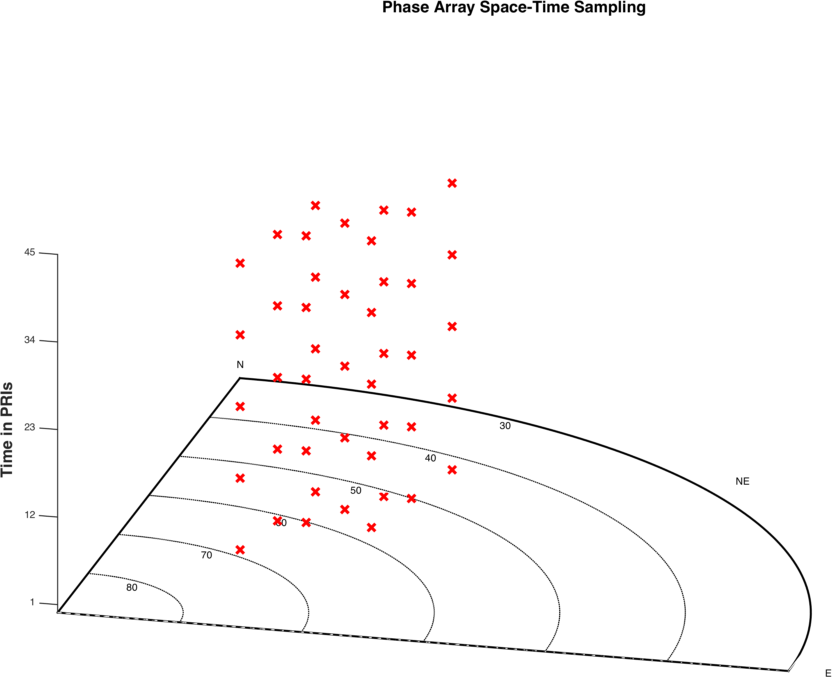
\includegraphics[width=5.5in]{phasedarraysts}
	\caption{Space-time sampling of the measurement space from Figure~\ref{fig:bp1} using a phased array based antenna, where the red x's mark the pulse in beam space and time. Beam positions from Figure \ref{fig:bp1} are shown below in blue at $z=0$.}	
	\label{fig:phbsts}
\end{figure}

The rapid steering ability of ESA systems relative to space-time sampling yields a new flexibility, in post processing, to statistically combine information from different beams using knowledge of the plasma velocity field, where this information is obtained either from external sources or from the Doppler shift of the ionospheric echoes themselves. This can help to relax the assumption of stationarity for plasmas that are evolving or changing their shape on time scales longer than the integration time. If the plasma moves into a different beam, returns from the same plasma can be integrated together with proper bookkeeping. This is contrary to the situation with dish antennas where returns from multiple plasma populations with different parameter sets are unavoidably averaged together.

In order to take advantage of new ESA flexibilities, this work puts forth the idea of the space-time ambiguity function. This concept extends the range ambiguity to all three spatial dimensions along with time. The goal of this paper is to develop a new formalism for treating space-time ambiguity for electronically steerable ISRs, and in particular ISRs that are capable of sampling a given volume on a pulse-by-pulse basis.   This paradigm can also be applied to other types of ISR system designs as well, but much of the utility of using this new formalism is more straightforwardly realized with ESA based systems.  An outline of the paper's development is as follows.  After developing the ambiguity formalism, we will develop specific cases of the impact of the three-dimensional ambiguity on moving plasma using conditions characteristic of polar cap patches. A simulation of a polar cap patch using a full ISR simulator, which creates ISR data at the I/Q level, will be shown. Lastly we will briefly discuss strategies that could improve measurements from electronically steerable ISR systems.

%%%%%%%%%%%%%% Ambiguity Derivation%%%%%%%%%%%%%%%%%%%%%%%%%%%%%%%

\section{Space-Time Ambiguity}

The space-time ambiguity can be thought of as a kernel to a combined volume and time integration operator. In the derivations that follow, we show that this ambiguity can be represented as a kernel operator in a Fredholm integral equation:

\begin{equation}
\label{eqn:friedholm}
\rho(\tau_s ,\mathbf{r}_{s},t_s) = \int L(\tau_s, \mathbf{r}_{s},t_s,\tau,\mathbf{r},t) R(\tau,\mathbf{r},t) dVd t d\tau
\end{equation}

\noindent where, for ISR, $L(\tau_s, \mathbf{r}_{s},t_s,\tau,\mathbf{r},t) $ is a blurring kernel over time and space, and $R(\tau,\mathbf{r},t) $ indicates the plasma medium's autocorrelation function at the lag $\tau$, time $t$, and position $\mathbf{r}$.

By using this formulation, many parallels between ISR and classic camera blurring problems can be made. In cameras, blurring can take place when an object moves over a space covered by one pixel while the shutter is open and the CCD is collecting photons. A diagram of this can be seen in Figure \ref{fig:ccd}. The same holds for the ISR measurement problem, except that the pixels are no longer square or continuous in Cartesian space and instead are determined by the beam shape and pulse pattern. This is shown in the diagrams in Figure \ref{fig:radarblur}.


\begin{figure}[h!]
\centering
	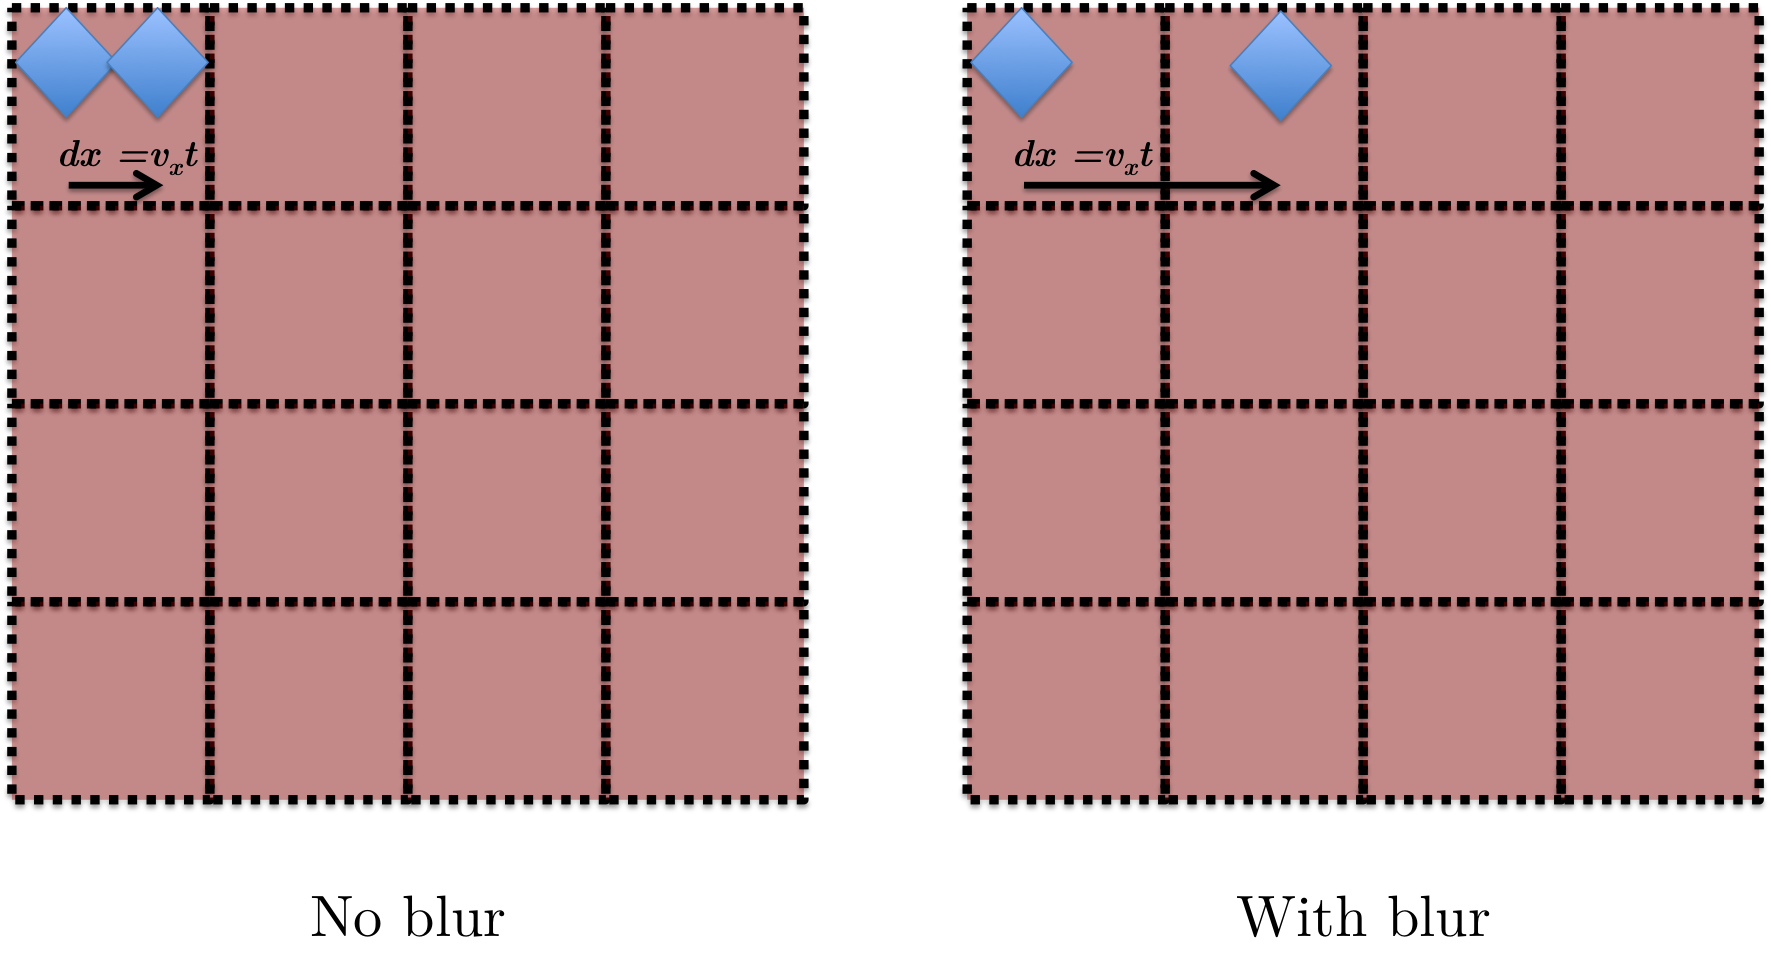
\includegraphics[height=3in]{ccddiagramall}
	\caption{CCD resolution cell diagram, showing cases where an object will be properly resolved and be blurred.}
	\label{fig:ccd}
\end{figure}

\begin{figure}[h!]
\centering
	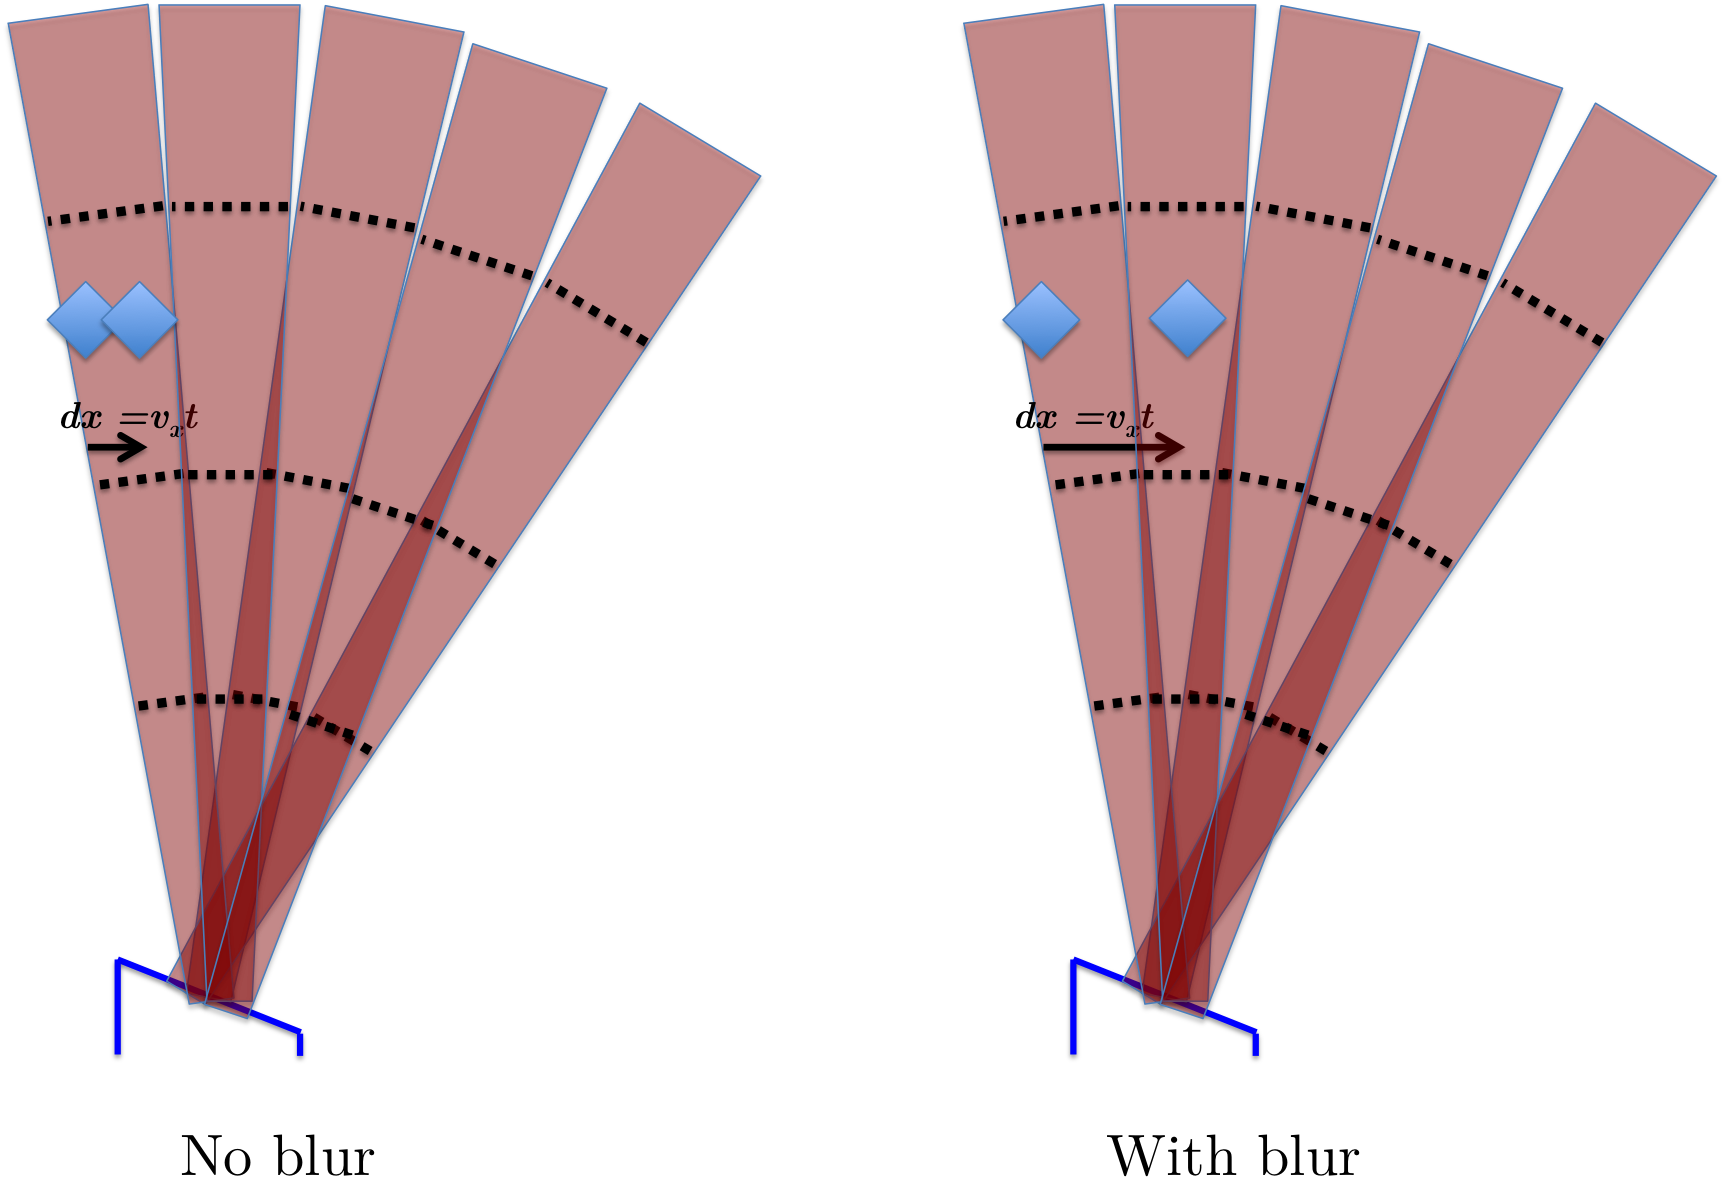
\includegraphics[height=3in]{radardiagramall}
	\caption{ISR resolution cell diagram, showing cases where an object will be properly resolved and be blurred.}
	\label{fig:radarblur}
\end{figure}

\subsection{Coordinate System Definitions}

Before we derive the full space-time ambiguity function, $L(\tau_s,\mathbf{r}_s,t_s,\tau,\mathbf{r},t)$, we will start with defining our coordinate system.  Our three dimensional coordinate system is defined as $\mathbf{r}=[x,y,z]^T$. For this coordinate system, $\mathbf{r}=[0,0,0]^T$ at the location of the radar and thus $r=|\mathbf{r}|$, also known as the range variable. This allows for the use of polar coordinates $\mathbf{r} =  [r,\theta_,\phi]^T$ where $\theta$ and $\phi$ are, respectively, the observer's elevation and azimuth angles.

The radar samples this space at a set of discrete points which will be referred to as $\mathbf{r}_s = [x_s,y_s,z_s]^T$ along with the discretized range expression $r_s=|\mathbf{r}_s|$. The sampled space consists of a number of points, composed of range gates within a beam multiplied by the number of beams. These points can also be referred in polar coordinates $\mathbf{r}_s = [r_s,\theta_s,\phi_s]^T$, where $\theta_s$  and $\phi_s$ are, respectively, the observationally sampled elevation and azimuth angles.

For notation purposes, we use two different sets of time commonly known in the hard-target radar literature as fast-time, $n$ and slow-time, $t$ \citep{richards:fundamentalsigproc}. Fast-time is used to describe processes with correlation time less than one PRI. Slow-time will be used for processes that decorrelate in time on the order of, or longer than, the system's PRI. In order to form estimates of ACFs with desired statistical properties, it is assumed that the plasma parameters parameters will change on the order of many tens to hundreds of PRIs in their stationary reference frame (i.e. remain wide sense stationary for this time). Generally, for incoherent scatter applications in the E-region of the ionosphere ($\approx$100 km altitude) and above, the decorrelation time is less than a PRI for systems with a center frequency in the UHF band, and thus ACFs must be formed over fast-time.

The terms $n$ and $t$ represent continuous variables, while $n_s$ and $t_s$ will be the fast time and slow time parameters sampled by the radar. The sampling rate of $n_s$ is set by the rate at which the system's A/D converters are run. The sampling of $t_s$ can, at the highest rate, be the PRI. At its lowest rate, it can be sampled once in a non-coherent processing interval (NCPI), or equivalently in a period of time it takes the radar to average the desired number of pulses for each beam. 

\subsection{Derivation}

The physical scattering mechanism underlying ISR produces measurable radar scatter from electron density fluctuations in the ionosphere, $n_e(\mathbf{r},n)$, at a specific wavenumber $\mathbf{k}$. These fluctuations scatter radio waves which can be observed by the receiver system of the radar \citep{dougherty:farley1960}. The emitted radar signal at the transmitter has a pulse shape $s(n)$ modulated at a central frequency creating a scattering wave number $\mathbf{k}$. Using the Born approximation, the signal received at time $n$, $x(n)$, can be represented as the following

\begin{equation}
\label{eq:xt}
x(n) = h(n) \ast \int \exp\left[-j\mathbf{k} \cdot \mathbf{r}\right]  s\left(n-\frac{2r}{c}\right) n_e(\mathbf{r},n) d\mathbf{r},
\end{equation}

\noindent where $h(n)$ is the receiver filter and the $\ast$ represents the convolution operator. In modern ISR systems, this signal $x(n)$ is then sampled at discrete points in fast-time which will be referred to as $n_s$. The convolution and sampling operation can be brought in the integral as the following,

\begin{equation}
\label{ex:xtaug}
x(n_s) = \int \exp\left[-j\mathbf{k} \cdot \mathbf{r}\right]  s\left(n-\frac{2r}{c}\right) n_e(\mathbf{r},n)h(n_s-n) d\mathbf{r}dn
\end{equation}


Once the signal has been received and sampled, the autocorrelation function is then estimated from the sampled signal $x(n_s)$. The full expression of the underlying autocorrelation of this signal is the following, 

\begin{multline}
\label{ex:acf0}
\langle x(n_s)x^*(n_s')\rangle =  \int \exp\left[-j \mathbf{k}\cdot \left(\mathbf{r}'-\mathbf{r} \right)\right]s\left(n-\frac{2r}{c}\right)s^*\left(n'-\frac{2r'}{c}\right) \\ h(n_s-n)h(n_s'-n')\langle n_e(\mathbf{r},n)n^*_e(\mathbf{r}',n')\rangle d\mathbf{r} d\mathbf{r}'dn dn',
\end{multline}

\noindent where $r'$ is the magnitude of the vector $\mathbf{r}'$. By assuming stationarity of second order signal statistics along fast time, we can then substitute the lag variables $\tau\equiv n'-n$, and $\tau_s\equiv n_s'-n_s$. With these substitutions, Equation \ref{ex:acf0} becomes


\begin{multline}
\label{ex:acf1}
\langle x(n_s)x^*(n_s+\tau_s)\rangle =\int \exp\left[-j \mathbf{k}\cdot \left(\mathbf{r}'-\mathbf{r} \right)\right]s\left(n-\frac{2r}{c}\right)s^*\left(n+\tau-\frac{2r'}{c}\right) \\ h(n_s-n)h(n_s+\tau_s-n-\tau) \langle n_e(\mathbf{r},n)n^*_e(\mathbf{r}',n+\tau)\rangle d\mathbf{r} d\mathbf{r}' dnd\tau
\end{multline}

\noindent We can make a simplifying assumption at this point that the space-time autocorrelation function of $n_e(\mathbf{r},t)$, $\langle n_e(\mathbf{r},n)n_e(\mathbf{r}',n+\tau)\rangle$, will go to zero as the magnitude of $\mathbf{y} \equiv \mathbf{r}'-\mathbf{r}$ increases beyond the debye length \citep{farley1969}. Thus, the rate which the spatial autocorrelation goes to zero will be such that $\tau\gg \frac{2||\mathbf{y}||}{c}$, allowing us to set $r= r'$ inside the arguments of $s$ and $h$. This allows Equation \ref{ex:acf1} to be rewritten as 
 
 \begin{multline}
 \label{ex:acf2}
 \langle x(n_s)x^*(n_s+\tau)\rangle = \int s\left(n-\frac{2r}{c}\right)s^*\left(n+\tau -\frac{2r}{c}\right) h(n_s-n)h^*(n_s+\tau_s-n-\tau) \\\left[\int \exp\left[-2j \mathbf{k}\cdot \mathbf{y}\right] \langle n_e(\mathbf{r},n)n^*_e(\mathbf{y}+\mathbf{r},n+\tau)\rangle d\mathbf{y} \right]drdn d\tau.
 \end{multline}

The inner integral is a spatial Fourier transform evaluated at the wave number of the radar $\mathbf{k}$. By again asserting stationarity along fast time, we can represent the true ACF as the following,
 \begin{equation}
 \label{eq:spft}
R(\tau,\mathbf{r})= \langle |n_e(\mathbf{k},r,\tau)|^2\rangle \equiv  \int \exp\left[-2j \mathbf{k}\cdot \mathbf{y} \right] \langle n_e(\mathbf{r},b)n^*_e(\mathbf{y}+\mathbf{r},n+\tau)\rangle d\mathbf{y}.
 \end{equation}
 
 \noindent Now Equation \ref{ex:acf2} becomes
 
 \begin{equation}
 \langle x(n_s)x^*(n_s+\tau_s)\rangle = \int \langle |n_e(\tau,\mathbf{k},\mathbf{r})|^2\rangle\left[\int s(n-\frac{2r}{c})s^*(n+\tau -\frac{2r}{c})h(n_s-n)h^*(n_s+\tau_s-n-\tau) dn \right]d\tau dr.
 \end{equation}

 If $n_s$ is replaced with $2r_s/c$ we can introduce the range ambiguity function $W(\tau_s,r_s,\tau,r)$ by doing the following substitution,
 \begin{equation}
 \label{eqn:rngamb}
 W(\tau_s,r_s,\tau,r)= \int s(n-\frac{2r}{c})s^*(n+\tau -\frac{2r}{c})h(2r_s/c-n)h^*(2r_s/c+\tau_s-n-\tau) dn.
 \end{equation}
 
Assuming, for the moment, that $R(\tau,\mathbf{r})$ only varies across the range dimension $r$, we can now represent this in the form of a Fredholm integral equation
 
 \begin{equation}
 \label{eqn:fredfirst}
 \langle x(2r_s/c)x^*(2r_s/c+\tau_s)\rangle = \int W(\tau_s,r_s,\tau,r)R(\tau,r) drd\tau.
 \end{equation}
 
\noindent The range ambiguity function, $W(\tau_s,r_s,\tau,r)$, can be thought of as a smoothing operator along the range and lag dimensions of $R(\tau,r)$. This result is also derived in \citet{nikoukar2008}, \citet{Woodman:1991is} and \cite{hysell2008}

 
The spatial ambiguity across azimuth and elevation angles is determined by the antenna beam pattern. In phased array antennas, this beam pattern is ideally the array factor multiplied by the element pattern \citep{Balanis:2005:ATA:1208379}. The array factor is determined by a number of things including the element spacing and the wave number of the radar, $k$. For example, by making idealized assumptions with no mutual coupling and that the array elements are simple cross dipole elements, AMISR systems will have the following antenna pattern for pointing angle ($\theta_s,\phi_s$): 

 \begin{equation}
 \label{eqn:amisrpat}
F(\theta_s,\phi_s,\theta,\phi) = \frac{1}{2}(1+\cos(\theta)^2)\left[ \frac{1}{MN} \left(1+\exp\left[j(\psi_y/2 + \psi_x)\right]\right)\frac{\sin((M/2) \psi_x)}{\sin(\psi_x)} \frac{\sin((N/2) \psi_x)}{\sin(\psi_x/2)}\right]^2,
 \end{equation}
 
 \noindent where $\psi_x = -k d_x(\sin\theta\cos\phi-\sin\theta_s\cos\phi_s)$, $\psi_y = -k d_y(\sin\theta\sin\phi-\sin\theta_s\sin\phi_s)$ and $M$ is the number of elements in the $x$ direction of the array, and $N$ is the number of elements in the $y$ direction(see Appendix: \ref{App:AMISRarr} for derivation).


The spatial ambiguity is a separable function made up of the components of $W(\tau_s,\tau,r_s,r)$ and $F(\theta_s,\phi_s,\theta,\phi)$. These two functions can be combined by multiplying the two, creating the spatial ambiguity function  $K(\tau_s,\mathbf{r}_s,\tau,\mathbf{r})$. This yields an expression for a single statistical realization of the ACF of the incoherent scatter random process, which will be referred to as $\rho(\tau_s,\mathbf{r}_s)$:


 \begin{align}
  \label{eqn:volume}
\rho(\tau_s,\mathbf{r}_s) &= \int F(\theta_s,\phi_s,\theta,\phi)W(\tau_s,r_s,\tau,r) R(\tau,\mathbf{r}) dV d\tau ,\\
	&= \int K(\tau_s,\mathbf{r}_s,\tau,\mathbf{r}) R(\tau,\mathbf{r})  dVd\tau.
\end{align}

A rendering of an example of this full spatial ambiguity function for an uncoded long pulse, with antenna pattern from Equation \ref{eqn:amisrpat} for four beams, can be seen in Figure \ref{fig:amb4}.

\begin{figure}
	\centering
	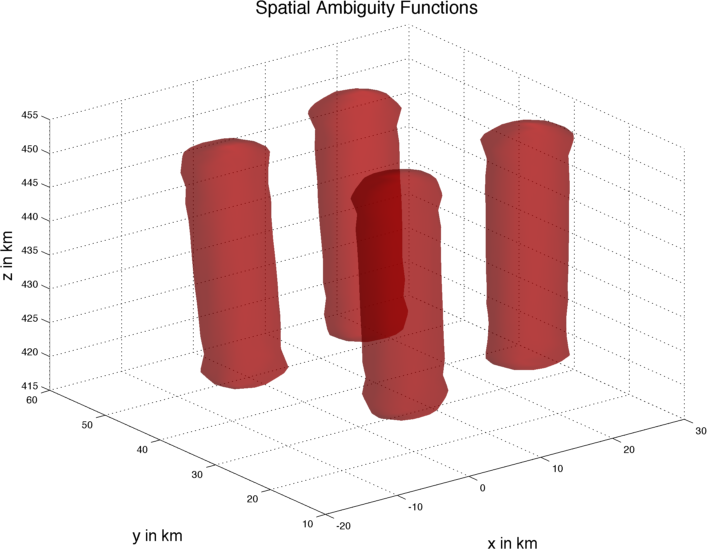
\includegraphics[width=5.5in]{spaceamb}
	\caption{Full spatial ambiguity function in Cartesian space for case with 4 beams with trailing edge of a 240$\mu$s pulse at 400km range. The surface represents the half power point of the ambiguity function.}	
	\label{fig:amb4}
\end{figure}

As mentioned above, this one pulse ACF estimate represents a single sample of a random process. In order to create a usable estimate, multiple samples of this ACF need to be averaged together to reduce the variance to sufficient levels in order to fit the estimate to a theoretical ACF that is a direct function of plasma parameter values. To show the impact of this averaging in creating the estimate of the ACF, we will add slow-time dependence to the expression for the medium ACF, which now becomes $R(\tau,\mathbf{r},t)$, and will also add another separable function $G(t_s,t)$ to the kernel. This function $G(t_s,t)$ can be thought of as a sampling and blurring kernel for the ACF if the plasma parameters change within an NCPI. Since the amount of time that the radar pulse is illuminating the plasma in a point of space is very short compared to the PRI, $G(t_s,t)$ can take the form of a summation of Dirac delta functions 

\begin{equation}
\label{eqn:Gexp}
G(t_s,t) = \displaystyle \sum_{j=0}^{J-1}\alpha_j \delta(t-t_s-jT_{REV}),
\end{equation}

\noindent where $J$ counts the number of pulses used over a NCPI, $T_{REV}$ is the amount of time it takes the radar to revisit the specific beam and $\alpha_j$ represent the weights that the radar assigns to the pulses. For systems using pulse-to-pulse steering, one strategy revisits each beam sequentially, in this case making $T_{REV}=N_{beam}T_{PRI}$, where $N_{beam}$ is the number of beams and $T_{PRI}$ is the PRI time period. For the case where weights are set to $1/J$, this operation simply averages the pulses. With Equation \ref{eqn:Gexp} incorporated into the overall ambiguity we obtain the full integral equation,

\begin{equation}
\label{eqn:sptamb}
	\rho(\tau_s,\mathbf{r}_s,t_s) =\int L(\tau_s,\mathbf{r}_s,t_s,\tau,\mathbf{r},t)R(\tau,\mathbf{r},t)dVdtd\tau.
\end{equation}

\noindent The final kernel, $L(\tau_s,\mathbf{r}_s,t_s,\tau,\mathbf{r},t) = G(t_s,t)K(\tau_s,\mathbf{r}_s,\tau,\mathbf{r})$, encompasses the full space-time ambiguity.

\subsection{Ambiguity after Frame Transformation}

We will now focus on the impact of the motion of plasma as it is going through the field of view of the radar. We will assume that the radar is integrating over a length of time $T$ beginning at $t_s$. The kernel $L$ will be represented as a separable function $K$ and $G$ as in Equation \ref{eqn:sptamb}. In this case, $G$ will be a summation of Dirac delta functions with weights of $1/J$. This will change Equation \ref{eqn:sptamb} to the following:

\begin{equation}
\label{eqn:L2}
\rho(\tau_s,\mathbf{r}_s,t_s) = \int K(\tau_s,\mathbf{r}_s,\tau,\mathbf{r}) \left[(1/J)\int_{t_s}^{t_s+T} \displaystyle \sum_{j=0}^{J-1} \delta(t-t_s-jT_{REV})R(\tau,\mathbf{r},t) dt\right] dVd\tau.
\end{equation}

Of specific interest in this study are instances in the high latitude ionosphere where embedded plasma structures are moving due to electric field drivers applied by the magnetosphere. In this case, it will be assumed that the plasma is a rigid object and will not deform with respect to $\mathbf{r}$ over time period $[t_0,t_0+T]$ where $T=JT_{REV}$ is the time for one NCPI. Also, it will be assumed that the plasma parcel moves with a constant velocity $\mathbf{v}$. Thus $R(\tau,\mathbf{r},t)\Rightarrow R(\tau,\mathbf{r}+\mathbf{v}t)$. The assumption of rigidity can in some cases be valid over the time period of the NCPI, on the order of a few minutes, while the plasma moves through the field of view of the radar. For example, in the high latitude ionosphere, large scale features in structures such as patches decay on the order of hours \citep{Tsunoda:1988ul}. This assumption is useful because it allows our framework to analyze impacts of these plasma variations on the parameter resolution of ISR systems. With these assumptions, Equation \ref{eqn:L2} becomes,

\begin{equation}
\label{eqn:L3}
\rho(\tau_s,\mathbf{r}_s,t_s) =(1/J) \int \int_{t_s}^{t_s+T} \displaystyle \sum_{j=0}^{J-1}\delta(t-t_s-jT_{REV}) K(\tau_s,\mathbf{r}_s,\tau,\mathbf{r})R(\tau,\mathbf{r}+\mathbf{v}t)dtdVd\tau\end{equation}

A change of variables to $\mathbf{r}' = \mathbf{r}+\mathbf{v}t$ acts as a Galilean transform and applies a warping to the kernel, changing the frame of reference. Since $R(\tau,\mathbf{r}')$ is no longer dependent on $t$, Equation \ref{eqn:L3} can be integrated in time and becomes:

\begin{equation}
\label{eqn:L5}
\rho(\tau_s,\mathbf{r}_s,t_s)= (1/J)\int \left[ \;\;  \displaystyle \sum_{j=0}^{J-1} K(\tau_s,\mathbf{r}_s,\tau,\mathbf{r}'-\mathbf{v}(t_s+jT_{REV})) \;\; \right]R(\tau,\mathbf{r}')dVd\tau.
\end{equation}

The problem can now be simplified further back to a Fredholm integral equation by simply replacing the terms in the square brackets as a new kernel $A(\tau_s,\mathbf{r}_s,t_s,\tau,\mathbf{r}')$:

\begin{equation}
\label{eqn:L6}
\rho(\tau_s,\mathbf{r}_s,t_s)= \int A(\tau_s,\mathbf{r}_s,t_s,\tau,\mathbf{r}') R(\tau,\mathbf{r}')dVd\tau.
\end{equation}

\noindent The impact of the plasma velocity on the ambiguity function can be seen in Figure \ref{fig:ambtime}. This is the same ambiguity as seen in Figure \ref{fig:amb4} but with a velocity of 500 m/s in the $y$ direction over a period of 2 minutes. This velocity creates a larger ambiguity function in the frame of reference of the moving plasma.
\begin{figure}[!t]
	\centering
	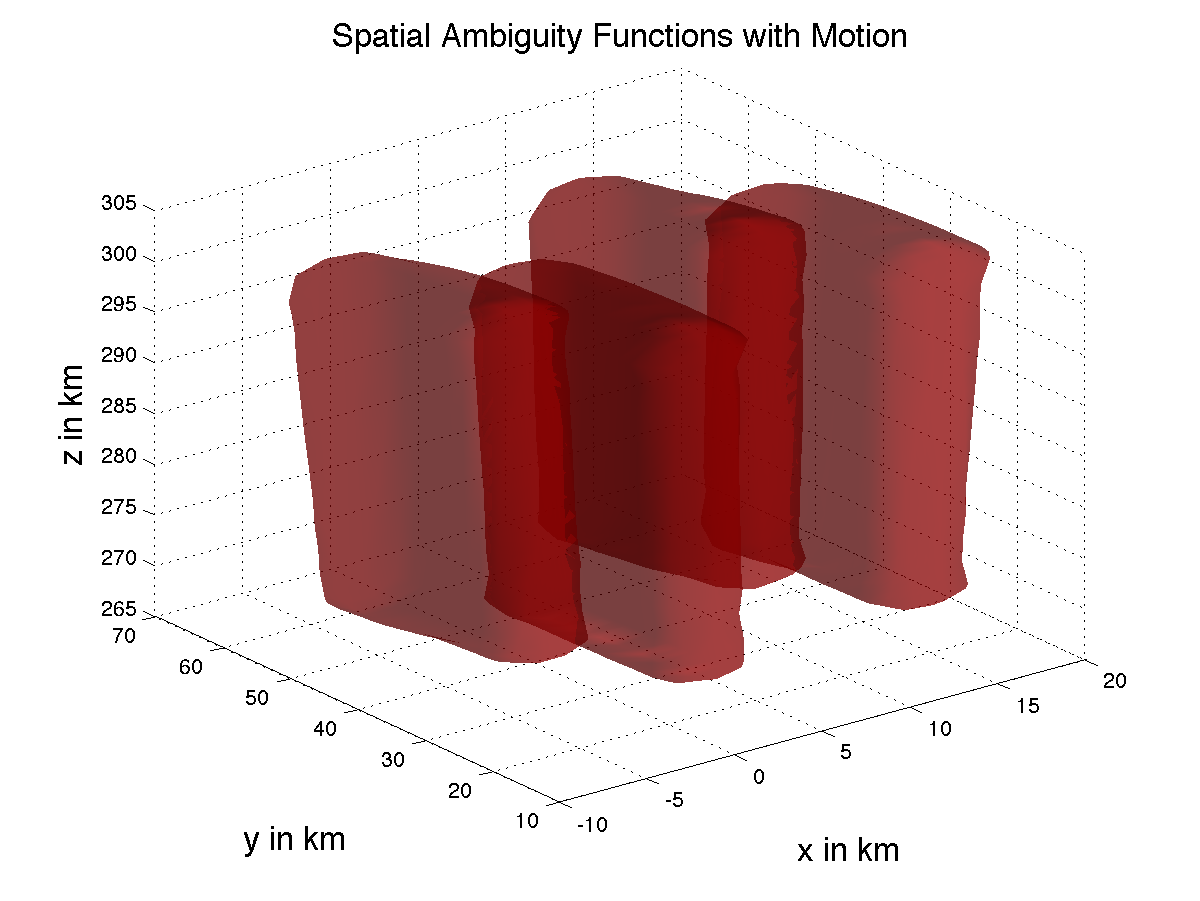
\includegraphics[width=5.5in]{spaceambmoving}
	\caption{Same spatial ambiguity as in Figure \ref{fig:amb4} but now with 500 m/s velocity in $y$ direction in plasma frame of reference. The surface represents the half power point of the ambiguity function.}
	\label{fig:ambtime}
\end{figure}

The operator $A$ can be determined through knowledge of the radar system's beam pattern along with the experiment's pulse pattern, integration time and inherent velocity of the plasma. This velocity $\mathbf{v}$ could be separately estimated by taking measurements of the Doppler shift by using a methodology like that seen in \citet{butler:imagingfregiondrifts}. With this strategy, the operator is now acting purely as a spatial blurring function instead of a full space-time function. We note that reducing dimensionality of the problem can make it easier to solve the inverse problem in practice.
%%%%%%%%%%%%%% Simulation %%%%%%%%%%%%%%%%%%%%%%%%%%%%%%%%%%%%%

\section{Simulation}

Although Figures \ref{fig:amb4} and \ref{fig:ambtime} show the spatial extent of the space-time ambiguity function both with and without target motion, the impact of this on the reconstruction data can better be shown through simulation. To do so, we present in this section data from a 3-D ISR simulator with a known set of ionospheric parameters. In the following section, we describe this simulator along with two case studies to show the impact of this ambiguity on properly reconstructing ionospheric plasma parameters.

\subsection{Simulator}
The 3-D ISR simulator creates data by deriving a time filter from the autocorrelation functions and applying them to complex white Gaussian noise generators. Stating this in another way, every point in time and space has a noise plant and filter structure as in Figure \ref{fig:IQdiagram}. The data is then scaled and summed together according to its location in range and angle space to radar. For this simulation, data points are only used if they are within 1.1 $^\circ$ of the center beam which is a simplification of the AMISR beam pattern. 

\begin{figure}[h!]
\centering
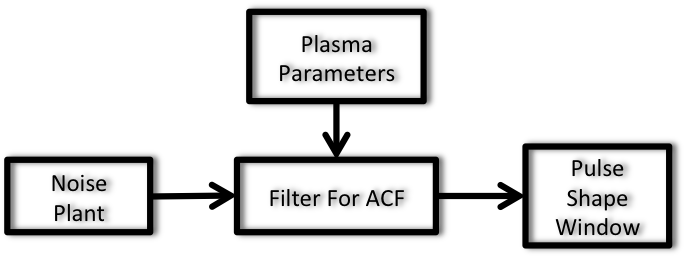
\includegraphics[width=4in]{diagrampart}
\caption{Diagram for I/Q simulator signal flow.}
\label{fig:IQdiagram}
\end{figure}

After the IQ data has been created it is processed to create estimates of the ACF at desired points of space. This processing follows a flow chart seen in Figure \ref{fig:chain}.

\begin{figure}[!t]
\centering
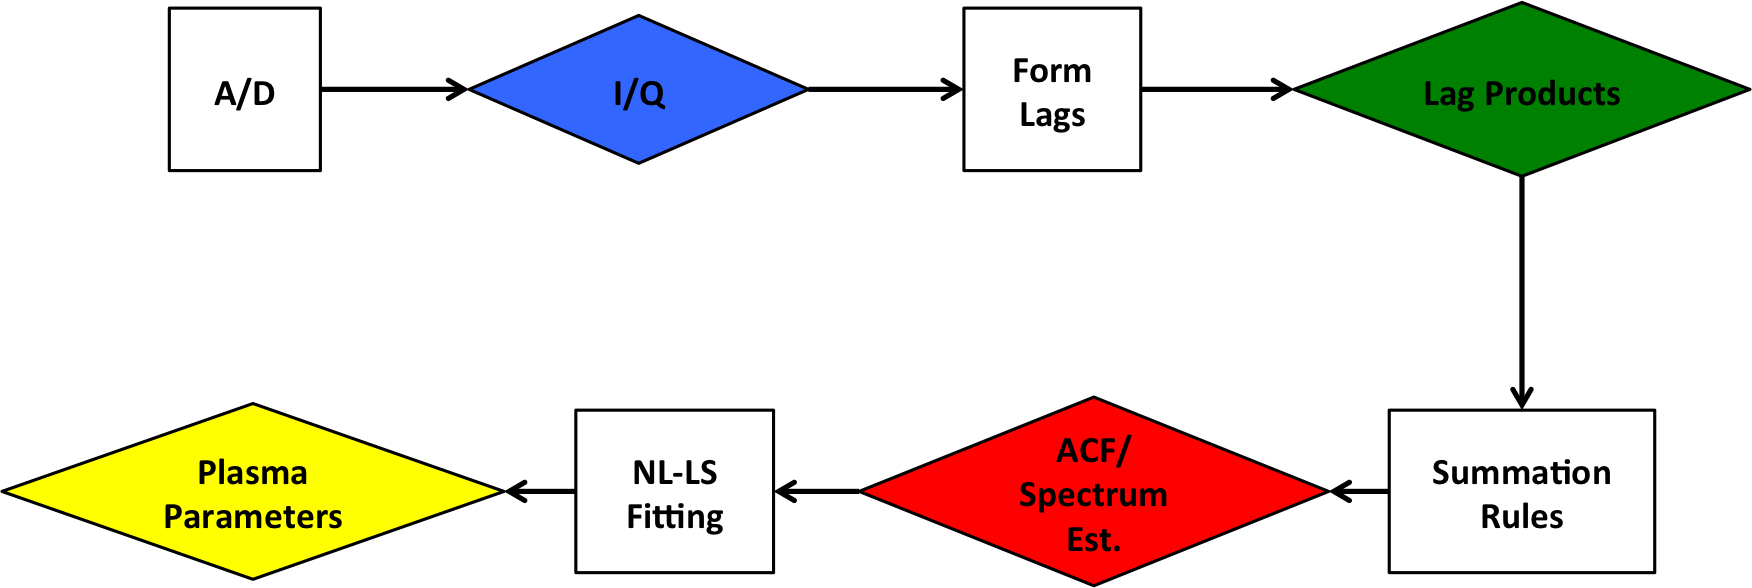
\includegraphics[width=6in]{datastackchain}
\caption{ISR signal processing chain, with signal elements as squares and data products as diamonds.}
\label{fig:chain}
\end{figure}

The sampled I/Q voltages can be represented as $x(n_s) \in\mathbb{C}^N$ where $N$ is the number of samples in a PRI.  At this point, the first step in estimating the autocorrelation function is taken.  For each range gate $m\in 0,1,...M-1$ an autocorrelation is estimated for each lag of $l \in 0,1...,L-1$.  This operation of forming the ACF estimates repeats for each pulse, $j\in 0,1,...J-1$, and is then summed over the $J$ pulses. The entire operation to form the initial estimate of $\hat{R}(m,l)$ is the following,

\begin{equation}
\label{lagpro}
\hat{R}(m,l) = \displaystyle\sum\limits_{j=0}^{J-1} x(m-\lfloor l/2\rfloor,j)x^*(m+\lceil l/2 \rceil,j).
\end{equation}


The case shown in Equation \ref{lagpro} is a centered lag product, which is what has been used for our simulations, but other types of lag product calculations are possible as well. In the centered lag product case, range gate index $m$ and sample index $n$ can be related by $m=n_s-\lfloor L/2\rfloor$ and the maximum lag and sample relation is $M=N-\lceil L/2 \rceil$. 

After the lag products have been formed, an estimate of the noise correlation is subtracted out of $\hat{R}(m,l)$, defined as $\hat{R}_w(m,l)$,

\begin{equation}
\label{lagpronoise}
\hat{R}_w(m_w,l) = \displaystyle\sum\limits_{j=0}^{J-1} w(m_w-\lfloor l/2\rfloor,j)w^*(m_w+\lceil l/2 \rceil,j),
\end{equation}

\noindent where $w(n_w)$ is the background noise process of the radar. 

The final estimate of the autocorrelation function after the noise subtraction and summation rule will be represented by $\hat{R}_f(m,l)$. At this point, a summation rule is applied and the data is sent off to be fit. The final parameters are derived through fitting these estimated ACFs with a standard Levenberg-Marquardt non-linear least-squares algorithm \citep{levenberg1944}, to ones that are determined using a theoretical model of the plasma ACF after application of the range ambiguity function. The simulations presented in this work use this methodology to produce plasma parameter scalar values of electron density, electron temperature, and ion temperature. To plot the three dimensional structures after fitting, we use a natural neighbor interpolation as seen in \citet{Semeter2009738}.


\subsection{Case 1: Electron Density Perturbation}

\begin{figure}
	\centering
	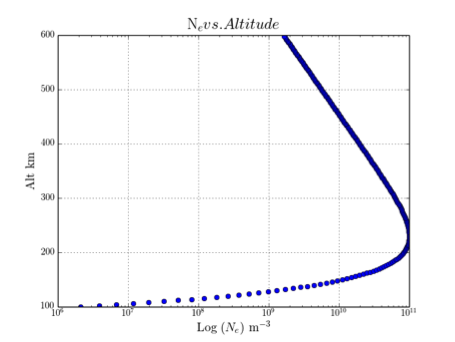
\includegraphics[width=4in]{nevsalt}
	\caption{Background electron density verses altitude profile used for simulations.}	
	\label{fig:nevsalt}
\end{figure}

\begin{figure}
	\centering
	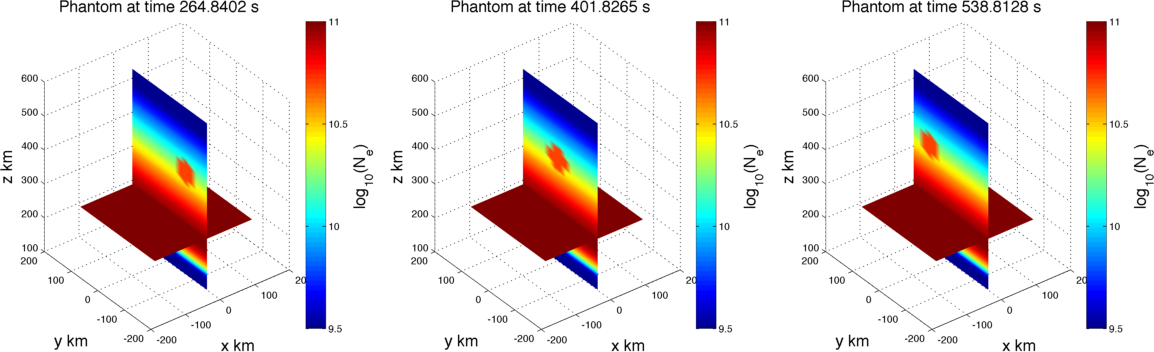
\includegraphics[width=6in]{phantom}
	\caption{Images of input $N_e$ for the simulation at three different times.}	
	\label{fig:phantom}
\end{figure}


The first example of the simulation described in the previous sections is a simple case of a small plasma enhancement moving through the radar field of view. This case is meant to model conditions expected in the polar cap ionosphere under southward IMF conditions \citep{Dahlgren:2012dq}. The background electron density is set to vary in altitude as a Chapman function, shown in Figure \ref{fig:nevsalt}, while the electron and ion temperature remains constant at 1000 K.

Embedded in the background density, we place a 35 km radius sphere of enhanced electron density of $5\times 10^{10} $ m$^{-3}$ centered at 400 km altitude and moving at 500 m/s velocity along the $\mathbf{y}$ direction. Images from this phantom can be seen in Figure \ref{fig:phantom}. To simplify the simulation, the ionospheric composition is assumed to be 100\% oxygen ions. For ease of comparison, the phantom is only shown in areas where it is in the radar's field of view. The positions of the 11 x 11 beam grid used for this case can be seen in Figure \ref{fig:beampattern}. 

Because only the electron density is varying, the fitting method in this case becomes simply a power estimate, as incoherent scatter theory predicts that  the electron density is directly proportional to the scattered power if the ion-to-electron temperature ratio is known. This example allows easier observation of the blurring from the space-time ambiguity function, while also demonstrating trade offs between statistical variance and blurring. 

Using the phantom, we can see how changing only the integration time can impact the reconstruction. In Figure \ref{fig:variable} we plot a case where only 10 pulses are used in each direction for the reconstruction, corresponding to an integration time of about 9 seconds. The enhancement can be seen as it moves through the field of view, although there is a high amount of variance in the reconstruction. Figure \ref{fig:blurred} shows the reconstruction with 200 pulses in each direction, or 3 minute total integration time. The variability has been reduced but there is a large amount of blurring of the enhancement as it moves through the field of view. 

\begin{figure}
	\centering
	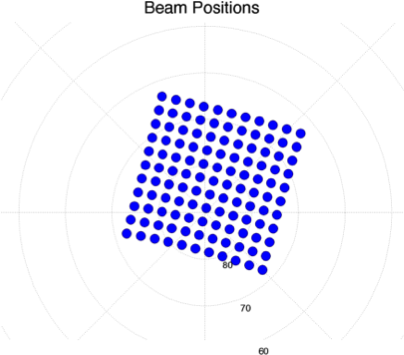
\includegraphics[width=4in]{beampattern}
	\caption{The 121 radar beam positions used in the simulations.}	
	\label{fig:beampattern}
\end{figure}

\begin{figure}
	\centering
	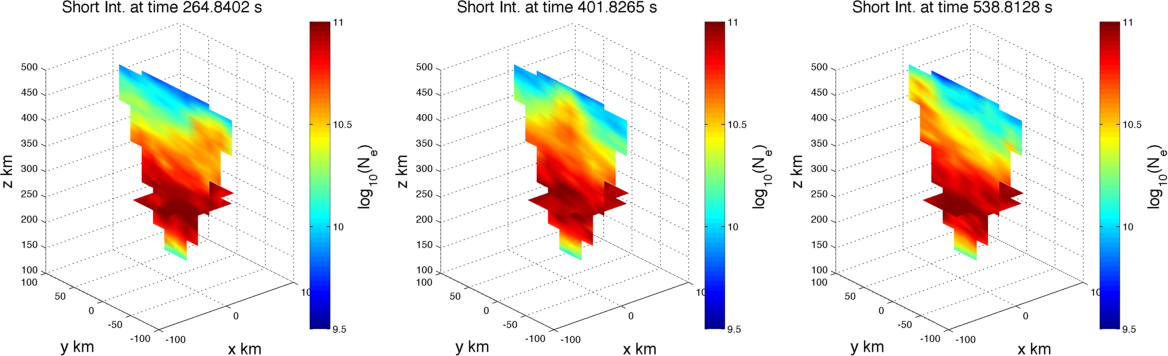
\includegraphics[width=6in]{variabledata}
	\caption{Reconstructions of $N_e$ using 10 pulses at three different times from the input shown in Figure \ref{fig:phantom}.}	
	\label{fig:variable}
\end{figure}


\begin{figure}
	\centering
	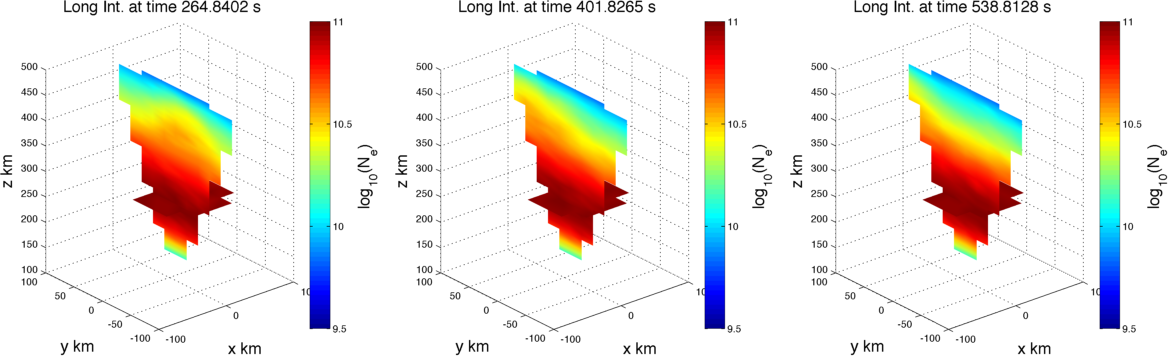
\includegraphics[width=6in]{blurreddata}
	\caption{Reconstructions of $N_e$ using 200 pulses at three different times from the input shown in Figure \ref{fig:phantom}.}	
	\label{fig:blurred}
\end{figure}

In order to give a comparison based on integration time, a phantom was also created with no motion. This can be seen in the first pane of Figure \ref{fig:statreconstruct}. An image using the same integration time as in Figure \ref{fig:variable} for the stationary phantom is shown as the center pane in Figure \ref{fig:statreconstruct}. Another image using the longer integration time (cf. Figure \ref{fig:blurred}) is plotted on the right pane of Figure \ref{fig:statreconstruct}. These images show that the blurring is on the same order from both integration times, in contrast to the case where the plasma is moving.

\begin{figure}
	\centering
	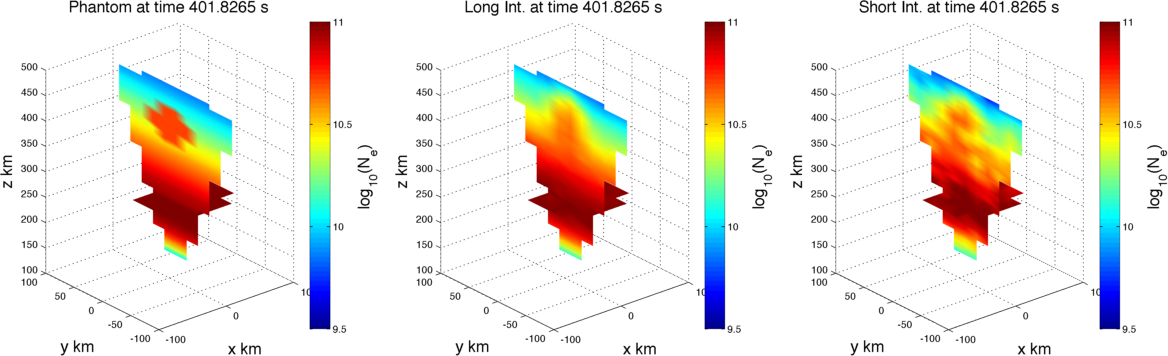
\includegraphics[width=6in]{stationary}
	\caption{Phantom of $N_e$ with no motion in plasma patch along with reconstructions using 10 and 200 pulses.}	
	\label{fig:statreconstruct}
\end{figure}

\subsection{Case 2: Plasma Temperature and Density Perturbation}
We present a second case of a simulation of the plasma density enhancement through the field of view, during which the ion and electron temperatures are allowed to vary. This case is a departure from the standard blurring problem seen in image processing, because the plasma parameters to be estimated are related to the observable ACF through a non-linear expression. However, the resulting ACF estimates are created through a linear blurring kernel in both time and space. 

We again use a plasma enhancement moving through the field of view at 500 m/s, but the electron and ion temperature varies with time and altitude. The  background ion and electron temperature vs. height can be seen in Figure \ref{fig:allparamsphantom}. As the electron density enhancement feature travels through the field of view, the ion and electron temperature is set to drop by the same ratio that the electron density is enhanced. This was done to add a variation in plasma temperatures along with electron density. 

\begin{figure}
	\centering
	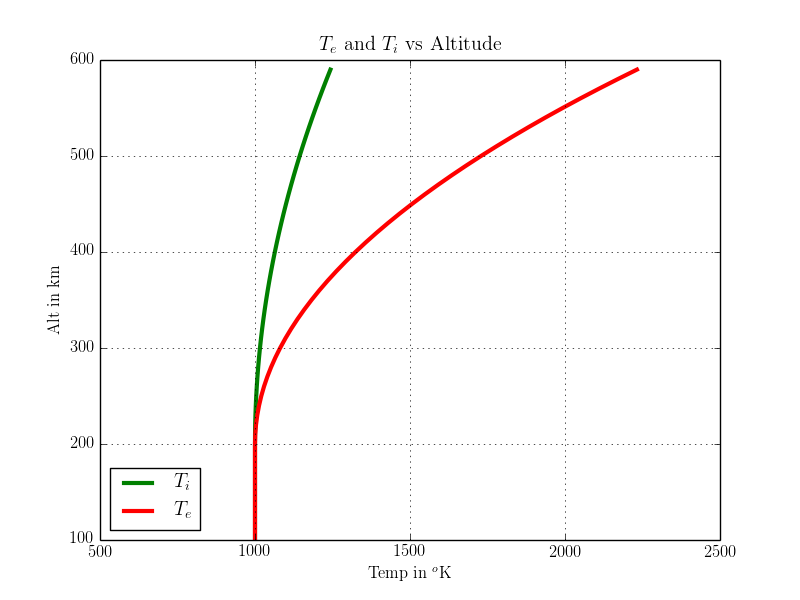
\includegraphics[width=4in]{tempvsheight}
	\caption{Background ion \& electron temperature verses height used for the simulation in case 2. }	
	\label{fig:allparamsphantom}
\end{figure}

The phantoms for each parameter at approximately 402 seconds can be seen in Figure \ref{fig:allparamsphantom}. The reconstruction of this field using a 3 minute integration time (200 pulses) centered at the same time can be seen in Figure \ref{fig:allparamsblurreddata}. Note that the reconstruction does not seem to show the electron density enhancement, even in a blurred form. 

\begin{figure}
	\centering
	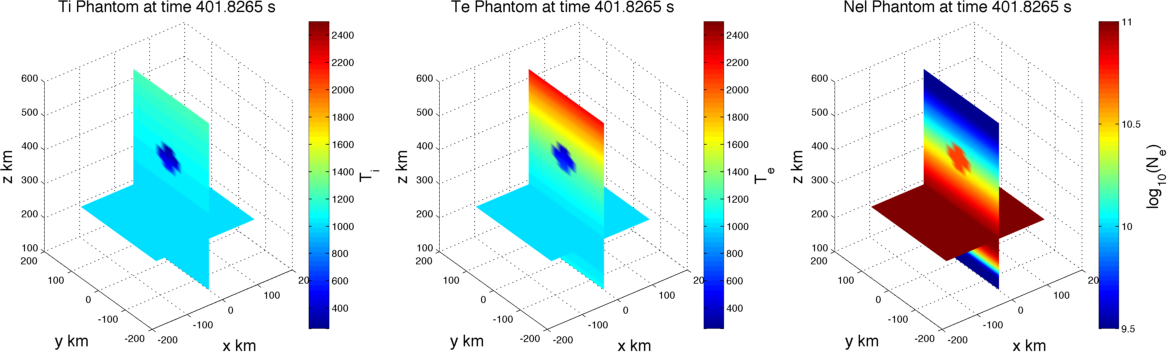
\includegraphics[width=6in]{allparamsphantom}
	\caption{Phantoms of $T_i$, $T_e$ and $N_e$ at $t=401.8265$s with a polar cap patch moving through the field of view.}	
	\label{fig:allparamsphantom}
\end{figure}

\begin{figure}
	\centering
	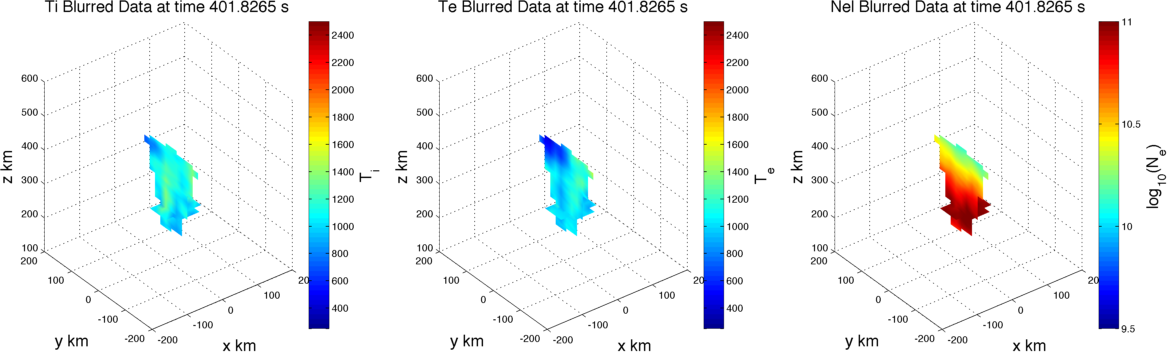
\includegraphics[width=6in]{allparamsblurreddata}
	\caption{Interpolated reconstructions of $T_i$, $T_e$ and $N_e$ from Figure \ref{fig:allparamsphantom} at $t=401.8265$s.}	
	\label{fig:allparamsblurreddata}
\end{figure}

In order to determine the reason behind the poor reconstruction, we look at the fit surface of one of the points in the reconstruction. The fit surface is the error between the estimated ISR spectrum and the spectrum derived from the different parameters. We will compare the points $\mathbf{r}=[10,10, 400]$ km and the closest reconstruction point in the radar field of view, $\mathbf{r}_s=[6.72,1.80, 398.77]$ at time 309.5s.  The time was chosen so the integrated measurement would be centered over the interval when the enhancement moved through this point, as the radar will integrate over two distinct plasma distributions. The plasma parameters at point $\mathbf{r}$ are $N_e=1.96\times 10^{10}$m$^{-3}$, $T_i =1064$ K and $T_e =1324$ K when there is no enhancement traveling through. When the enhancement is traveling through this point $N_e=5\times 10^{10}$m$^{-3}$, $T_i =416$ K and $T_e =518$ K. The speed of the enhancement, 500 m/s, causes about two-thirds of the pulses measured to correspond to the enhanced plasma during the integration.

After integrating and fitting the ISR spectra, the parameter fit results at $\mathbf{r}$ are $N_e=2.36\times 10^{10}$m$^{-3}$, $T_i =973$ K and $T_e =500$ K, representative of neither the background or enhanced plasma. To investigate further, the fit surface was formed over the parameter space of $N_e =1\times 10^{10}$ to $1\times10^{11} $m$^{-3}$, and for both $T_e$ and $T_i$ over values 100 to 1500 K. In this case, the fit surface showed that the global minimum was located in the same location as found by the Levenberg-Marquardt algorithm. A two dimensional cut of the fit surface variation as a function of $T_i$ and $T_e$ holding $N_e=2.43\times 10^{10} $m$^{-3}$ is shown in Figure \ref{fig:fitsurface}. The final fit values are located at a global minimum, indicating that this is not a result of multiple parameter ambiguities but rather that the non uniformity of the plasma parameters caused an erroneous fit. Mixtures of different plasma populations causing erroneous fits have been shown before, such as in \citet{knudsen1993} where a shear flow perpendicular to the radar beam apparently caused poor reconstruction of plasma parameters. 

\begin{figure}
	\centering
	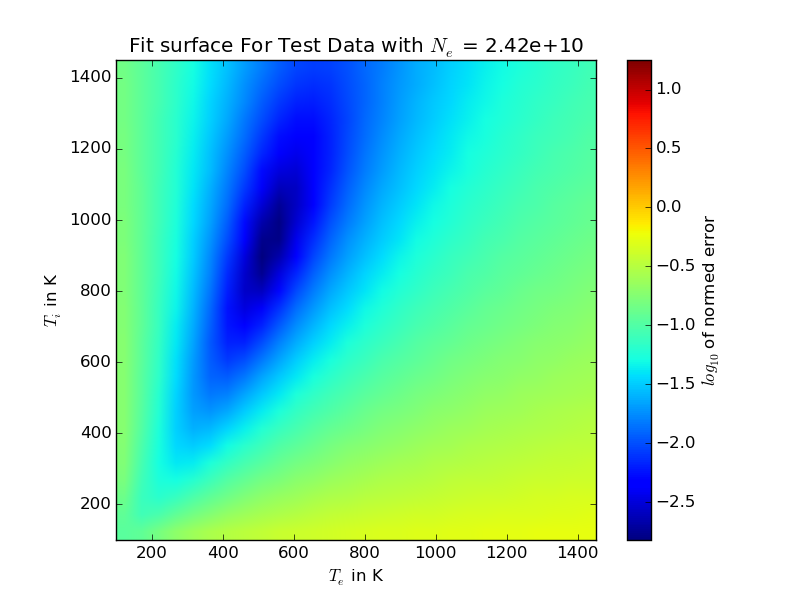
\includegraphics[width=6in]{Fitsurface3}
	\caption{Fit surface from spectrum estimated at $\mathbf{r}_s=[6.72,1.80, 398.77]$ and $t$ = 309.5s.}	
	\label{fig:fitsurface}
\end{figure}

For further insight, power spectra calculated from the original known plasma parameters compared with those calculated from the final fit estimates can be seen in Figure \ref{fig:spectrums}. In this case, the spectrum estimated from the data has been reduced by averaging over time and space which has lowered its power dramatically, thus creating an ambiguous shape which also matches a spectrum with improper parameter values.

\begin{figure}
	\centering
	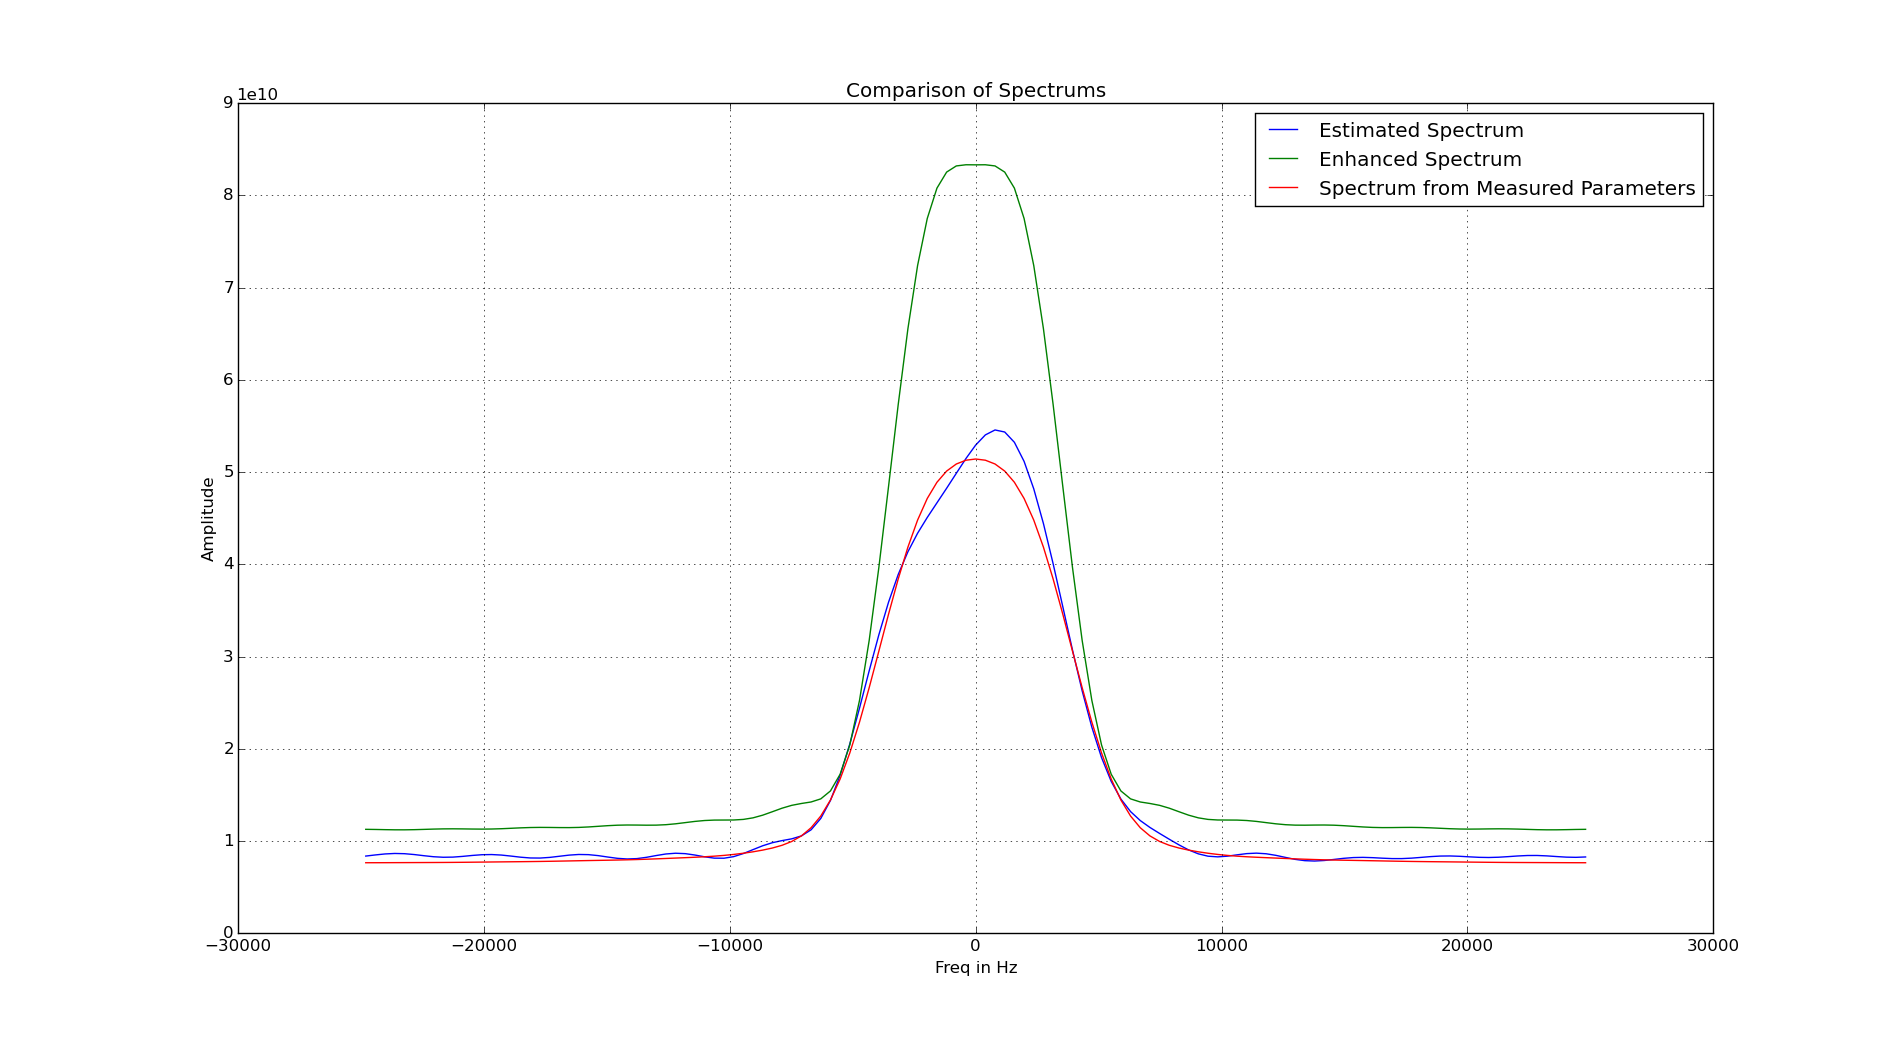
\includegraphics[width=6in]{spectrums}
	\caption{Estimated spectrum from $\mathbf{r}_s=[6.72,1.80, 398.77]$ along with spectrum from measured parameters and from enhanced plasma.}	
	\label{fig:spectrums}
\end{figure}
%%%%%%%%%%%%%% Mitigation %%%%%%%%%%%%%%%%%%%%%%%%%%%%%%%%%%%%%

\section{Possible Mitigation Techniques}

As can be seen from the previous sections, a number of different types of errors can occur if the ISR measurement technique does not properly account for the full space-time ambiguity function under ionospheric variability conditions. There are a number of possible approaches one could take in order to mitigate these effects and produce an improved data product from electronically scanned ISR measurements.  The discussion in this section is by no means exhaustive, but rather gives an idea of the utility of this frame work. In order to focus the discussion, we will concentrate on methods to remove motion blur type errors that occur when plasma is moving through the field of view, along with techniques to improve the spatio-temporal resolution of the measurements.

In order to reduce the impact from plasma parcel motion, a relatively simple approach would involve processing the data in the frame of reference of the moving density field. The convection velocity is manifested as a bulk Doppler shift in the ISR spectrum.  Under the uniform composition assumptions applied in our examples, this Doppler shift is independent of the other parameters, and so $\mathbf{v}$ in Equation \ref{eqn:L5}  could be extracted using the separate analysis described by \citet{RDS:RDS5552} and \citet{butler:imagingfregiondrifts}. After measuring the velocity, instead of integrating data across slow-time in the same beam, one could integrate across different beams using this knowledge, assuming one corrects for differences in flow angle that would impact the bulk Doppler offset. This would allow a statistically stationary ACF to be formed from plasma populations with the same physical state as they move through the field of view.

To improve the plasma parameter resolution, it may also be necessary to perform some sort of regularization. There are two types of regularization that can be applied in this case.  The first type is parameter based regularization, such as is employed in full profile analysis \citep{RDS:RDS3308,hysell2008}. We will use the term parameter based regularization in this case since the procedure applies constraints to the physical parameters that are determined after fitting. Full profile analysis has only been applied to date along the range dimension and not in all three spatial dimensions. However, if full profile analysis is extended so it can be used in ESA systems, a forward model between the actual ACF and the one measured in the radar would be needed. This model formulation is encompassed within Equation \ref{eqn:sptamb}.  

The second regularization method is referred to here as data based regularization. This term infers the application of constraints first to the estimates of the autocorrelation functions, after which fitting takes place. The constraints usually deal with how the data itself changes over time and space by constraining the energy of the ACF \citep{Virtanen:2008vx, nikoukar2008} or its derivative \citep{nikoukar:thesis}. A simplified description of the data based regularization lies in an equivalence with a deconvolution operation on the ACFs. This has an advantage that one can use linear inverse theory to estimate ACF lags before fitting, as opposed to parameter based regularization schemes such as full profile analysis where ionospheric parameters are directly estimated and regularized. Because of these features, data based regularization has the advantage of generally being more computationally tractable than parameter based.  However, a significant drawback to data based regularization is that is very difficult to argue what constraint would be "correct" to use, while in full profile analysis the constraints are often based on likely physical variations in the ionosphere. In any case, in order to extend the methodology from \citet{Virtanen:2008vx} and \citet{ nikoukar2008}, one can use the kernel $L$ for the case of improving measurements from an ESA ISR.





%%%%%%%%%%%%%% Conclusion %%%%%%%%%%%%%%%%%%%%%%%%%%%%%%%%%%%%

\section{Conclusion}This publication has laid the foundation for the optimal analysis of volumetric data acquired from electronically steerable ISR systems. The framework developed here takes into account the full antenna beam pattern, pulse pattern and time integration. Through simulations, we have shown how plasma motion can impact reconstruction of parameters which, compounded with the non-linear nature of the parameter fitting step, can create errors which are potentially unexpected and hard to predict. Lastly, we briefly outlined a number of possible mitigation approaches improving measurements derived from ESA ISRs.

\appendix
\section{Derivation of Idealized AMISR Array Pattern} \label{App:AMISRarr}
The current antenna on the AMISR systems is made up 8x16 set of panel of half wave cross dipoles. Each panel has 32 cross dipoles in a 8x4 hexagonal configuration. In the current set up at the Poker Flat site this yields at 4096 element array in a 64x64 element hexagonal configuration.

In order to simplify the antenna can be treated as two rectangular arrays of cross dipoles interleaved together. In the $x$ direction each of these arrays will have a spacing of $2d_x$ with $M/2$ elements. The $y$ direction will be of length $N$ elements and spacing $d_y$. Using basic planar phase array theory, \citep{Balanis:2005:ATA:1208379}, the pattern from the first array can be represented as 

\begin{equation}
\label{eqn:arrpat1}
E_1(\theta,\phi) =\displaystyle \sum_{m=1}^{M/2}\sum_{n=1}^{N} \exp\left[-j2\left(m-1\right)kd_x\sin\theta\cos\phi -j\left(n-1\right) k d_y\sin\theta\sin\phi\right].
\end{equation}

\noindent Since the second array can be though of a shifted version of the first in the $x$ and $y$ directions we get the following

\begin{equation}
\label{eqn:arrpat2}
E_2(\theta,\phi) =\displaystyle \sum_{m=1}^{M/2}\sum_{n=1}^{N} \exp\left[-j\left(2m-1\right)kd_x\sin\theta\cos\phi -j\left(n-1/2\right) k d_y\sin\theta\sin\phi\right].
\end{equation}

In order to simplify notation we will make the following substitutions, $\psi_x = -k d_x\sin\theta\cos\phi$, $\psi_y = -k d_y\sin\theta\sin\phi$. Using Equations \ref{eqn:arrpat1} and \ref{eqn:arrpat2} we can see the following relationship,

\begin{equation}
\label{eqn:arrpateqn}
\begin{split}
E_2(\theta,\phi)  &=  \exp\left[j(\psi_y/2 + \psi_x)\right] E_1(\theta,\phi)  \\&= \exp\left[j(\psi_y/2 + \psi_x)\right]  \displaystyle \sum_{m=1}^{M/2}\sum_{n=1}^{N}  \exp\left[-j2\left(m-1\right) \psi_x -j\left(n-1\right) \psi_y\right].
\end{split}
\end{equation}

\noindent Adding $E_1$ and $E_2$ together we get the following linear array pattern

\begin{equation} \label{eq1}
\begin{split}
E(\theta,\phi) &= \displaystyle  \left(1+ \exp\left[j(\psi_y/2 + \psi_x)\right]\right)\sum_{m=1}^{M/2}\sum_{n=1}^{N}  \exp\left[-j2\left(m-1\right) \psi_x -j\left(n-1\right) \psi_y\right].\\
& = \frac{1}{MN} \left(1+ \exp\left[j(\psi_y/2 + \psi_x)\right]\right)\frac{\sin((M/2) \psi_x)}{\sin(\psi_x)} \frac{\sin((N/2) \psi_x)}{\sin(\psi_x/2)}.
\end{split}
\end{equation}

Since the array is steerable this can be taken into account in the equations by simply changing the definitions of $\psi_x $ and $\psi_y$ to $\psi_x = k d_x(\sin\theta\cos\phi-\sin\theta_s\cos\phi_s)$, and $\psi_y = k d_y(\sin\theta\sin\phi-\sin\theta_s\sin\phi_s)$. Lastly the antenna pattern of a single cross dipole can be represented as $ \frac{1}{2}(1+\cos^2(\theta))$\citep{Balanis:2005:ATA:1208379}. By taking the squared magnitude of the array factor and multiplying it with the pattern of the dipole we get Equation \ref{eqn:amisrpat},

\begin{equation}
\label{eqn:amisrpatfinal}
F(\theta_s,\phi_s,\theta,\phi) = \frac{1}{2}(1+\cos(\theta)^2)\left| \frac{1}{MN} \left(1+ \exp\left[j(\psi_y/2 + \psi_x)\right]\right)\frac{\sin((M/2) \psi_x)}{\sin(\psi_x)} \frac{\sin((N/2) \psi_x)}{\sin(\psi_x/2)}\right|^2.
\end{equation}
 
 \begin{acknowledgments}
This work was supported by the National Science Foundation, through Aeronomy Program Grant AGS-1339500 to Boston University and Cooperative Agreement AGS-1242204 between the NSF and the Massachusetts Institute of Technology, and by the Air Force Office of Scientific Research under contract FA9550-12-1-018.   The authors are grateful to the International Space Science Institute (ISSI, Bern, Switzerland) for sponsoring a series of workshops from which the idea for this work emerged. 

Software used to create figures for this publications can be found at https://github.com/jswoboda/Spacetimeisrambcode. Please contact the corresponding author, John Swoboda at swoboj@bu.edu, with any questions regarding the software along with any requests for the specific data used for the figures. \end{acknowledgments}
 
\bibliographystyle{BibTeX/agufull08}
\bibliography{BibTeX/litreview}



\end{article}

\end{document}
